\section{Procedure}
In this section we present the procedure that was followed to trap a polaron in rutile. We start with a standard calculation on a rutile unit cell, followed by a DFT+U calculation. Then, we trap an extra electron in a supercell. We compute the properties of the polaron investigating the DOS and band structure. The calculation of a delocalized electron is discussed as well, and the two solutions are compared.
\subsection{DFT and DFT+U calculation on rutile}
We begin by performing a standard DFT calculation on rutile. To do so, we first need some information on the material we are investigating.

Rutile has a tetragonal unit cell, with two titanium and four oxygen atoms inside. A sketch of a unit cell is given in \cref{fig:rutile}.
\begin{figure}
    \centering
    \begin{subfigure}[t]{0.48\textwidth}
        \centering
        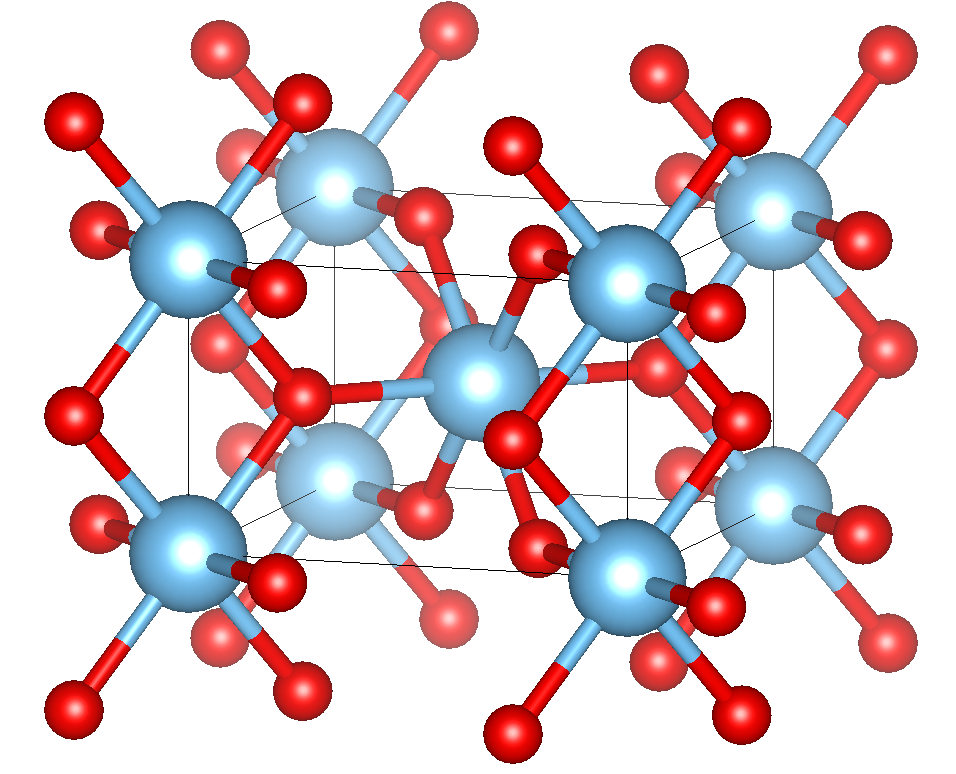
\includegraphics[width=1\textwidth]{figures/rutile.png}
        \caption{Unit cell}
        \label{fig:rutile}
    \end{subfigure}
    \hfill
    \begin{subfigure}[t]{0.48\textwidth}
        \centering
        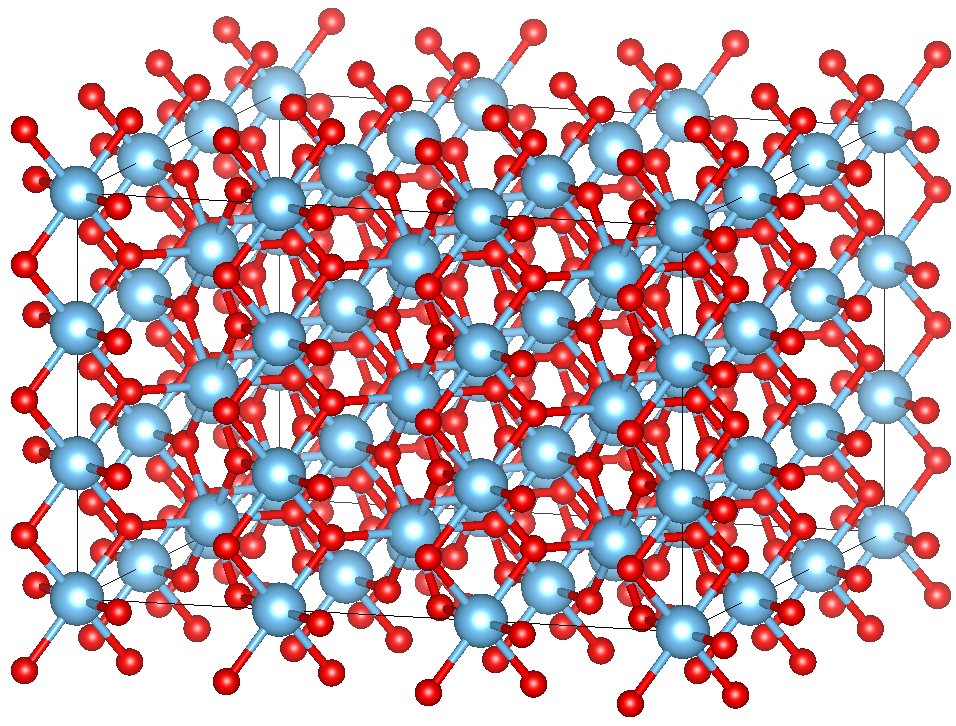
\includegraphics[width=1\textwidth]{figures/supercell.png}
        \caption{$3\times3\times3$ supercell}
        \label{fig:supercell}
    \end{subfigure}
    \caption[Rutile unit cell and supercell]{Rutile unit cell and supercell. Titanium is blue and oxygen is red. The images have been rendered with Vesta \cite{zotero-174}.}
\end{figure}
The lattice parameters and the positions of the atoms were taken from The Materials Project website \cite{Jain2013} and inserted in the  POSCAR file. The properties of the atoms, as we discussed in \cref{sec:implementation}, are given by the pseudopotentials. For Ti, a projector augmented wave (PAW) pseudopotential with 12 electrons was used, whereas for O a PAW pseudopotential with 6 electrons was chosen. Finally, a k-points grid was generated. We chose to use a $\Gamma$-centered grid with points separated by \SI{0.03}{\angstrom^{-1}}. For rutile unit cell, this is achieved by a
$7\times7\times11$ grid. The necessary file was generated using Vaspkit \cite{VASPKIT}.

With these settings, a series of DFT calculations was performed. In all the calculation we used a cut-off energy of \SI{700}{eV}. The convergence was stopped when the energy difference of two successive electronic calculations was smaller than \SI{1e-8}{eV} and the forces on the ions smaller than \SI{0.01}{eV/\angstrom}. A Gaussian smearing with $\sigma = 0.05$ was used for the calculations that involved the relaxation of the system or the computation of the band structure. For the computation of the DOS, the tetrahedron method was chosen. In fact, the tetrahedron method usually gives better results, but it is not applicable to calculations where the position of the ions changes or with non-uniform k-points grids.

Before investigating the electronic properties of the material, we wanted to be sure that the structure we used was properly relaxed. A non-spin-polarized calculation was performed on the unit cell allowing the relaxation of the ions positions. The volume and the shape of the unit cell was kept constant, allowing the atomic positions to change. This is generally achieved by performing a series of standard electronic DFT calculations. Once, the electronic charge converges, the forces on the ions is computed. The ions are then moved accordingly, minimizing the forces that act on them. Then, the next electronic calculation is run. The process stops once both the electronic and ionic calculations converge.

The relaxed structure was then used for a standard self-consistent DFT calculation. In particular, the DOS, the electronic charge density and the wavefunctions were computed. The result was used in a non-selfconsistent calculation to compute the band structure. The bands were calculated along a special path of k-points. Conventionally, these points are named  $\Gamma$-X-M-$\Gamma$-Z-R-A-Z; X-R; M-A. They are high-symmetry points of the first Brillouin zone of a tetragonal system. The position of the points in the Brillouin zone is displayed in \cref{fig:symmetry_points}. Each high-symmetry k-point was connected with a line of 10 k-points to the next one.

\begin{figure}
    \centering
    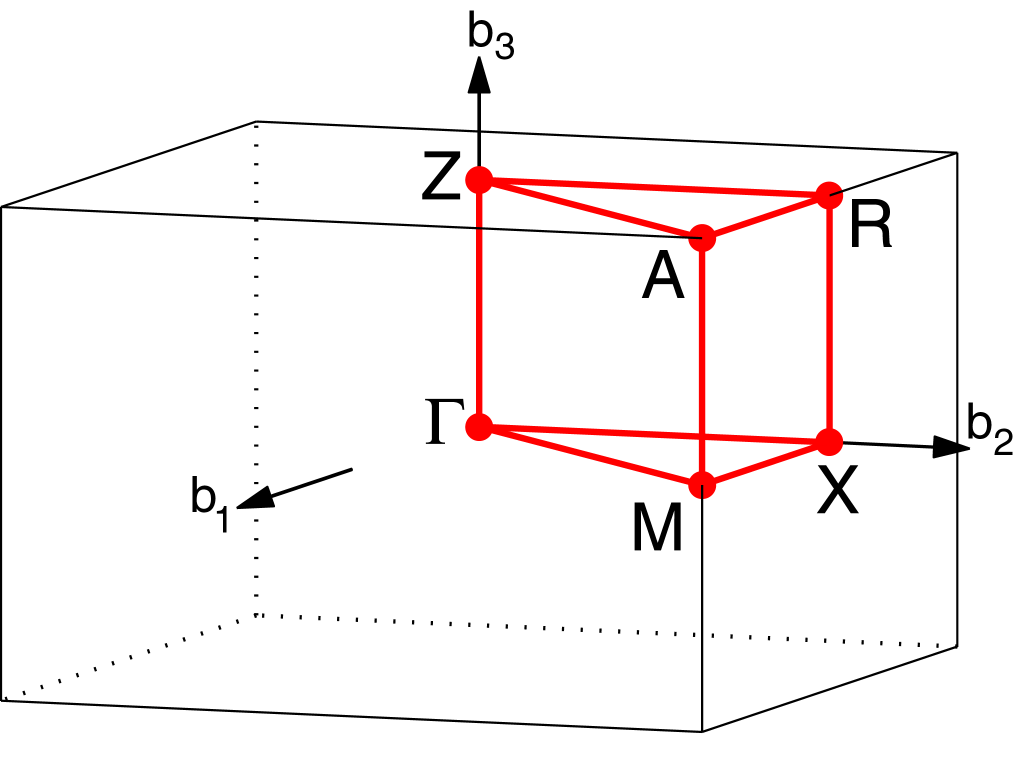
\includegraphics[width=0.5\textwidth]{figures/brillouin_zone}
    \caption[Brillouin zone of a tetragonal system]{Brillouin zone of a tetragonal system, the red path passes through the high-symmetry points of the zone. $\vec{b}_1, \vec{b}_2, \vec{b}_3$ are the reciprocal base vectors of a tetragonal unit cell. The path used in the calculation of the band structure was $\Gamma$-X-M-$\Gamma$-Z-R-A-Z; X-R; M-A.}
    \label{fig:symmetry_points}
\end{figure}

As discussed in \cref{sec:dft+u}, DFT often fails to give appropriate results in band-gap calculations. To correct the problem, the previous calculations were repeated in the DFT+U approach.  The DFT+U correction was implemented following the Duradev approach, setting the value of U to \SI{3.9}{eV} \cite{reticcioli2022}. The correction was applied to the d-orbitals of titanium, leaving the other orbitals unaltered. Starting from the relaxed structure, we relaxed it again with the DFT+U correction. The DOS and band structure were computed as well, following the same procedure described above.

\subsection{Electron localization}
To find a polaronic solution, we had to add an extra electron to the system and localize it at the center of the cell. Since the electron must be localized in a region of the size of a unit cell, the simulation cannot be run on a unit cell alone. Since the unit cell is repeated in the crystal, the polaron would interfere with itself at the cell boundaries, resulting in self-interaction errors. To solve this problem, the unit cell is replaced with a supercell, which is a cell made by the repetition of a unit cell. For this reason, only small polarons can be simulated in DFT. For large polarons, the supercell size would be too big to be simulated.

A $3\times3\times3$ supercell was created with the Vesta software \cite{zotero-174}, repeating the relaxed unit cell three times in each direction. A sketch of the supercell is reported in \cref{fig:supercell}. The unit cell that was repeated was the result of the relaxation performed with the DTF+U correction. The usual calculations described above were performed on the supercell, computing the DOS and the band structure. Moreover, the number of electrons present in the system was noted. Knowing the number of electrons is useful to trap an extra electron in the supercell.

Since the formation of the polaron is only slightly energetically favored compared to a delocalized solution, the extra electron is difficult to localize. Simply adding one electron to the system does not result in a localized state. The electron enters the conduction band, and it is delocalized in the whole cell.

To find a localized solution, a more gradual approach was necessary. To add an electron to the system, the central titanium atom was substituted with vanadium. Vanadium is the element following titanium in the periodic table, so it has one more electron and a stronger nuclear attraction. The substitution was done modifying the POSCAR and POTCAR files. For vanadium, a PAW pseudopotential with 13 electrons was used.

Added the electron, a number of expedients was needed to ensure that the electron was localized. The aim was to localize it on the central atom, the vanadium one. The six oxygen atoms around the central atom were moved outwards by \SI{0.04}{\angstrom}, creating a potential well for the electron. Moreover, the $U-J$ value was set to \SI{3.9}{eV} for titanium d-orbitals and to \SI{9}{eV} for vanadium d-orbitals. Together, the stronger nuclear attraction of the vanadium atom, the displacement of the oxygen atoms, and the high $U-J$ value, favored the electron localization at the center of the supercell.

A DFT+U calculation was run allowing lattice relaxations.  The extra electron in the system introduced a spin magnetic moment, so the calculation was spin-polarized. The magnetic moment was initially set to zero for every atom except for the vanadium one, which was set to $+\mu_B$, where $\mu_B$ is the Bohr magneton. To check if the electron was localized, the magnetic moment of the atoms was read in the output. For a localized state, we expected the central vanadium atom to be the only one with a magnetic moment (of 0.7-0.9 $\mu_B$).

The localized solution was used to initialize a new set of calculations. The goal was to gradually substitute the vanadium atom with a high $U-J$ value with a titanium atom with a normal $U-J$ value. This was done in two steps.

Firstly, vanadium was removed and titanium was placed back, leaving
the $U-J$ value applied to the central atom unchanged. To keep the electron in the system, the number of electrons was manually set to the same number of the calculation with vanadium. The atomic positions were set as in the previous calculations, with the oxygen atoms shifted by \SI{0.04}{\angstrom}. The calculation was initialized with the charge density and wavefunctions obtained from the system with vanadium, where the electron was already localized.

A new DFT+U calculation with lattice relaxation was run. The calculation was spin-polarized, and the initial magnetic moment was read from the charge density file. The localization of the electron was checked looking at the magnetic moment as explained above. Moreover, the eigenvalues and DOS were also inspected to see if a new state was present in the middle of the band gap.

Secondly, the calculation of the polaron was done continuing the last calculation with a normal $U-J$ value for the central titanium atom. The calculation was initialized with the atomic positions, charge density and wavefunctions of the previous calculation. The magnetic moments, DOS and eigenvalues were inspected again to check if the polaron was still present.

\subsection{Polaron}

Some last calculations were run to compute the polaron properties. An electronic calculation without relaxation was done starting from the previous result to compute a more precise DOS. The band structure of the polaronic solution was also computed with a non-self-consistent calculation on the usual path of k-points. Finally, the isosurfaces of the charge density of the polaron was computed. To do so, the charge was decomposed over the different bands, and the polaronic band was selected restricting the calculation to an appropriate energy interval. The final result was rendered with Vesta, and the electron localization observed.

A delocalized solution was computed as well for comparison. To achieve this, an extra electron was added to the supercell and a non-spin-polarized DFT+U calculation was performed. The extra electron was added manually, setting the number of electrons to the number of the electrons in the original rutile supercell plus one. The DOS and band structure were computed as usual.